\documentclass{report}

%%%%%%%%%%%%%%%%%%%%%%%%%%%%%%%%%
% PACKAGE IMPORTS
%%%%%%%%%%%%%%%%%%%%%%%%%%%%%%%%%


\usepackage[tmargin=2cm,rmargin=1in,lmargin=1in,margin=0.85in,bmargin=2cm,footskip=.2in]{geometry}
\usepackage{amsmath,amsfonts,amsthm,amssymb,mathtools}
\usepackage[varbb]{newpxmath}
\usepackage{xfrac}
\usepackage[makeroom]{cancel}
\usepackage{mathtools}
\usepackage{bookmark}
\usepackage{enumitem}
\usepackage{hyperref,theoremref}
\hypersetup{
	pdftitle={Assignment},
	colorlinks=true, linkcolor=doc!90,
	bookmarksnumbered=true,
	bookmarksopen=true
}
\usepackage[most,many,breakable]{tcolorbox}
\usepackage{xcolor}
\usepackage{varwidth}
\usepackage{varwidth}
\usepackage{etoolbox}
%\usepackage{authblk}
\usepackage{nameref}
\usepackage{multicol,array}
\usepackage{tikz-cd}
\usepackage[ruled,vlined,linesnumbered]{algorithm2e}
\usepackage{comment} % enables the use of multi-line comments (\ifx \fi) 
\usepackage{import}
\usepackage{xifthen}
\usepackage{pdfpages}
\usepackage{transparent}

\newcommand\mycommfont[1]{\footnotesize\ttfamily\textcolor{blue}{#1}}
\SetCommentSty{mycommfont}
\newcommand{\incfig}[1]{%
    \def\svgwidth{\columnwidth}
    \import{./figures/}{#1.pdf_tex}
}

\usepackage{tikzsymbols}
\renewcommand\qedsymbol{$\Laughey$}


%\usepackage{import}
%\usepackage{xifthen}
%\usepackage{pdfpages}
%\usepackage{transparent}


%%%%%%%%%%%%%%%%%%%%%%%%%%%%%%
% SELF MADE COLORS
%%%%%%%%%%%%%%%%%%%%%%%%%%%%%%



\definecolor{myg}{RGB}{56, 140, 70}
\definecolor{myb}{RGB}{45, 111, 177}
\definecolor{myr}{RGB}{199, 68, 64}
\definecolor{mytheorembg}{HTML}{F2F2F9}
\definecolor{mytheoremfr}{HTML}{00007B}
\definecolor{mylenmabg}{HTML}{FFFAF8}
\definecolor{mylenmafr}{HTML}{983b0f}
\definecolor{mypropbg}{HTML}{f2fbfc}
\definecolor{mypropfr}{HTML}{191971}
\definecolor{myexamplebg}{HTML}{F2FBF8}
\definecolor{myexamplefr}{HTML}{88D6D1}
\definecolor{myexampleti}{HTML}{2A7F7F}
\definecolor{mydefinitbg}{HTML}{E5E5FF}
\definecolor{mydefinitfr}{HTML}{3F3FA3}
\definecolor{notesgreen}{RGB}{0,162,0}
\definecolor{myp}{RGB}{197, 92, 212}
\definecolor{mygr}{HTML}{2C3338}
\definecolor{myred}{RGB}{127,0,0}
\definecolor{myyellow}{RGB}{169,121,69}
\definecolor{myexercisebg}{HTML}{F2FBF8}
\definecolor{myexercisefg}{HTML}{88D6D1}


%%%%%%%%%%%%%%%%%%%%%%%%%%%%
% TCOLORBOX SETUPS
%%%%%%%%%%%%%%%%%%%%%%%%%%%%

\setlength{\parindent}{1cm}
%================================
% THEOREM BOX
%================================

\tcbuselibrary{theorems,skins,hooks}
\newtcbtheorem[number within=section]{Theorem}{Theorem}
{%
	enhanced,
	breakable,
	colback = mytheorembg,
	frame hidden,
	boxrule = 0sp,
	borderline west = {2pt}{0pt}{mytheoremfr},
	sharp corners,
	detach title,
	before upper = \tcbtitle\par\smallskip,
	coltitle = mytheoremfr,
	fonttitle = \bfseries\sffamily,
	description font = \mdseries,
	separator sign none,
	segmentation style={solid, mytheoremfr},
}
{th}

\tcbuselibrary{theorems,skins,hooks}
\newtcbtheorem[number within=chapter]{theorem}{Theorem}
{%
	enhanced,
	breakable,
	colback = mytheorembg,
	frame hidden,
	boxrule = 0sp,
	borderline west = {2pt}{0pt}{mytheoremfr},
	sharp corners,
	detach title,
	before upper = \tcbtitle\par\smallskip,
	coltitle = mytheoremfr,
	fonttitle = \bfseries\sffamily,
	description font = \mdseries,
	separator sign none,
	segmentation style={solid, mytheoremfr},
}
{th}


\tcbuselibrary{theorems,skins,hooks}
\newtcolorbox{Theoremcon}
{%
	enhanced
	,breakable
	,colback = mytheorembg
	,frame hidden
	,boxrule = 0sp
	,borderline west = {2pt}{0pt}{mytheoremfr}
	,sharp corners
	,description font = \mdseries
	,separator sign none
}

%================================
% Corollery
%================================
\tcbuselibrary{theorems,skins,hooks}
\newtcbtheorem[number within=section]{Corollary}{Corollary}
{%
	enhanced
	,breakable
	,colback = myp!10
	,frame hidden
	,boxrule = 0sp
	,borderline west = {2pt}{0pt}{myp!85!black}
	,sharp corners
	,detach title
	,before upper = \tcbtitle\par\smallskip
	,coltitle = myp!85!black
	,fonttitle = \bfseries\sffamily
	,description font = \mdseries
	,separator sign none
	,segmentation style={solid, myp!85!black}
}
{th}
\tcbuselibrary{theorems,skins,hooks}
\newtcbtheorem[number within=chapter]{corollary}{Corollary}
{%
	enhanced
	,breakable
	,colback = myp!10
	,frame hidden
	,boxrule = 0sp
	,borderline west = {2pt}{0pt}{myp!85!black}
	,sharp corners
	,detach title
	,before upper = \tcbtitle\par\smallskip
	,coltitle = myp!85!black
	,fonttitle = \bfseries\sffamily
	,description font = \mdseries
	,separator sign none
	,segmentation style={solid, myp!85!black}
}
{th}


%================================
% LENMA
%================================

\tcbuselibrary{theorems,skins,hooks}
\newtcbtheorem[number within=section]{Lenma}{Lenma}
{%
	enhanced,
	breakable,
	colback = mylenmabg,
	frame hidden,
	boxrule = 0sp,
	borderline west = {2pt}{0pt}{mylenmafr},
	sharp corners,
	detach title,
	before upper = \tcbtitle\par\smallskip,
	coltitle = mylenmafr,
	fonttitle = \bfseries\sffamily,
	description font = \mdseries,
	separator sign none,
	segmentation style={solid, mylenmafr},
}
{th}

\tcbuselibrary{theorems,skins,hooks}
\newtcbtheorem[number within=chapter]{lenma}{Lenma}
{%
	enhanced,
	breakable,
	colback = mylenmabg,
	frame hidden,
	boxrule = 0sp,
	borderline west = {2pt}{0pt}{mylenmafr},
	sharp corners,
	detach title,
	before upper = \tcbtitle\par\smallskip,
	coltitle = mylenmafr,
	fonttitle = \bfseries\sffamily,
	description font = \mdseries,
	separator sign none,
	segmentation style={solid, mylenmafr},
}
{th}


%================================
% PROPOSITION
%================================

\tcbuselibrary{theorems,skins,hooks}
\newtcbtheorem[number within=section]{Prop}{Proposition}
{%
	enhanced,
	breakable,
	colback = mypropbg,
	frame hidden,
	boxrule = 0sp,
	borderline west = {2pt}{0pt}{mypropfr},
	sharp corners,
	detach title,
	before upper = \tcbtitle\par\smallskip,
	coltitle = mypropfr,
	fonttitle = \bfseries\sffamily,
	description font = \mdseries,
	separator sign none,
	segmentation style={solid, mypropfr},
}
{th}

\tcbuselibrary{theorems,skins,hooks}
\newtcbtheorem[number within=chapter]{prop}{Proposition}
{%
	enhanced,
	breakable,
	colback = mypropbg,
	frame hidden,
	boxrule = 0sp,
	borderline west = {2pt}{0pt}{mypropfr},
	sharp corners,
	detach title,
	before upper = \tcbtitle\par\smallskip,
	coltitle = mypropfr,
	fonttitle = \bfseries\sffamily,
	description font = \mdseries,
	separator sign none,
	segmentation style={solid, mypropfr},
}
{th}


%================================
% CLAIM
%================================

\tcbuselibrary{theorems,skins,hooks}
\newtcbtheorem[number within=section]{claim}{Claim}
{%
	enhanced
	,breakable
	,colback = myg!10
	,frame hidden
	,boxrule = 0sp
	,borderline west = {2pt}{0pt}{myg}
	,sharp corners
	,detach title
	,before upper = \tcbtitle\par\smallskip
	,coltitle = myg!85!black
	,fonttitle = \bfseries\sffamily
	,description font = \mdseries
	,separator sign none
	,segmentation style={solid, myg!85!black}
}
{th}



%================================
% Exercise
%================================

\tcbuselibrary{theorems,skins,hooks}
\newtcbtheorem[number within=section]{Exercise}{Exercise}
{%
	enhanced,
	breakable,
	colback = myexercisebg,
	frame hidden,
	boxrule = 0sp,
	borderline west = {2pt}{0pt}{myexercisefg},
	sharp corners,
	detach title,
	before upper = \tcbtitle\par\smallskip,
	coltitle = myexercisefg,
	fonttitle = \bfseries\sffamily,
	description font = \mdseries,
	separator sign none,
	segmentation style={solid, myexercisefg},
}
{th}

\tcbuselibrary{theorems,skins,hooks}
\newtcbtheorem[number within=chapter]{exercise}{Exercise}
{%
	enhanced,
	breakable,
	colback = myexercisebg,
	frame hidden,
	boxrule = 0sp,
	borderline west = {2pt}{0pt}{myexercisefg},
	sharp corners,
	detach title,
	before upper = \tcbtitle\par\smallskip,
	coltitle = myexercisefg,
	fonttitle = \bfseries\sffamily,
	description font = \mdseries,
	separator sign none,
	segmentation style={solid, myexercisefg},
}
{th}

%================================
% EXAMPLE BOX
%================================

\newtcbtheorem[number within=section]{Example}{Example}
{%
	colback = myexamplebg
	,breakable
	,colframe = myexamplefr
	,coltitle = myexampleti
	,boxrule = 1pt
	,sharp corners
	,detach title
	,before upper=\tcbtitle\par\smallskip
	,fonttitle = \bfseries
	,description font = \mdseries
	,separator sign none
	,description delimiters parenthesis
}
{ex}

\newtcbtheorem[number within=chapter]{example}{Example}
{%
	colback = myexamplebg
	,breakable
	,colframe = myexamplefr
	,coltitle = myexampleti
	,boxrule = 1pt
	,sharp corners
	,detach title
	,before upper=\tcbtitle\par\smallskip
	,fonttitle = \bfseries
	,description font = \mdseries
	,separator sign none
	,description delimiters parenthesis
}
{ex}

%================================
% DEFINITION BOX
%================================

\newtcbtheorem[number within=section]{Definition}{Definition}{enhanced,
	before skip=2mm,after skip=2mm, colback=red!5,colframe=red!80!black,boxrule=0.5mm,
	attach boxed title to top left={xshift=1cm,yshift*=1mm-\tcboxedtitleheight}, varwidth boxed title*=-3cm,
	boxed title style={frame code={
					\path[fill=tcbcolback]
					([yshift=-1mm,xshift=-1mm]frame.north west)
					arc[start angle=0,end angle=180,radius=1mm]
					([yshift=-1mm,xshift=1mm]frame.north east)
					arc[start angle=180,end angle=0,radius=1mm];
					\path[left color=tcbcolback!60!black,right color=tcbcolback!60!black,
						middle color=tcbcolback!80!black]
					([xshift=-2mm]frame.north west) -- ([xshift=2mm]frame.north east)
					[rounded corners=1mm]-- ([xshift=1mm,yshift=-1mm]frame.north east)
					-- (frame.south east) -- (frame.south west)
					-- ([xshift=-1mm,yshift=-1mm]frame.north west)
					[sharp corners]-- cycle;
				},interior engine=empty,
		},
	fonttitle=\bfseries,
	title={#2},#1}{def}
\newtcbtheorem[number within=chapter]{definition}{Definition}{enhanced,
	before skip=2mm,after skip=2mm, colback=red!5,colframe=red!80!black,boxrule=0.5mm,
	attach boxed title to top left={xshift=1cm,yshift*=1mm-\tcboxedtitleheight}, varwidth boxed title*=-3cm,
	boxed title style={frame code={
					\path[fill=tcbcolback]
					([yshift=-1mm,xshift=-1mm]frame.north west)
					arc[start angle=0,end angle=180,radius=1mm]
					([yshift=-1mm,xshift=1mm]frame.north east)
					arc[start angle=180,end angle=0,radius=1mm];
					\path[left color=tcbcolback!60!black,right color=tcbcolback!60!black,
						middle color=tcbcolback!80!black]
					([xshift=-2mm]frame.north west) -- ([xshift=2mm]frame.north east)
					[rounded corners=1mm]-- ([xshift=1mm,yshift=-1mm]frame.north east)
					-- (frame.south east) -- (frame.south west)
					-- ([xshift=-1mm,yshift=-1mm]frame.north west)
					[sharp corners]-- cycle;
				},interior engine=empty,
		},
	fonttitle=\bfseries,
	title={#2},#1}{def}



%================================
% Solution BOX
%================================

\makeatletter
\newtcbtheorem{question}{Question}{enhanced,
	breakable,
	colback=white,
	colframe=myb!80!black,
	attach boxed title to top left={yshift*=-\tcboxedtitleheight},
	fonttitle=\bfseries,
	title={#2},
	boxed title size=title,
	boxed title style={%
			sharp corners,
			rounded corners=northwest,
			colback=tcbcolframe,
			boxrule=0pt,
		},
	underlay boxed title={%
			\path[fill=tcbcolframe] (title.south west)--(title.south east)
			to[out=0, in=180] ([xshift=5mm]title.east)--
			(title.center-|frame.east)
			[rounded corners=\kvtcb@arc] |-
			(frame.north) -| cycle;
		},
	#1
}{def}
\makeatother

%================================
% SOLUTION BOX
%================================

\makeatletter
\newtcolorbox{solution}{enhanced,
	breakable,
	colback=white,
	colframe=myg!80!black,
	attach boxed title to top left={yshift*=-\tcboxedtitleheight},
	title=Solution,
	boxed title size=title,
	boxed title style={%
			sharp corners,
			rounded corners=northwest,
			colback=tcbcolframe,
			boxrule=0pt,
		},
	underlay boxed title={%
			\path[fill=tcbcolframe] (title.south west)--(title.south east)
			to[out=0, in=180] ([xshift=5mm]title.east)--
			(title.center-|frame.east)
			[rounded corners=\kvtcb@arc] |-
			(frame.north) -| cycle;
		},
}
\makeatother

%================================
% Question BOX
%================================

\makeatletter
\newtcbtheorem{qstion}{Question}{enhanced,
	breakable,
	colback=white,
	colframe=mygr,
	attach boxed title to top left={yshift*=-\tcboxedtitleheight},
	fonttitle=\bfseries,
	title={#2},
	boxed title size=title,
	boxed title style={%
			sharp corners,
			rounded corners=northwest,
			colback=tcbcolframe,
			boxrule=0pt,
		},
	underlay boxed title={%
			\path[fill=tcbcolframe] (title.south west)--(title.south east)
			to[out=0, in=180] ([xshift=5mm]title.east)--
			(title.center-|frame.east)
			[rounded corners=\kvtcb@arc] |-
			(frame.north) -| cycle;
		},
	#1
}{def}
\makeatother

\newtcbtheorem[number within=chapter]{wconc}{Wrong Concept}{
	breakable,
	enhanced,
	colback=white,
	colframe=myr,
	arc=0pt,
	outer arc=0pt,
	fonttitle=\bfseries\sffamily\large,
	colbacktitle=myr,
	attach boxed title to top left={},
	boxed title style={
			enhanced,
			skin=enhancedfirst jigsaw,
			arc=3pt,
			bottom=0pt,
			interior style={fill=myr}
		},
	#1
}{def}



%================================
% NOTE BOX
%================================

\usetikzlibrary{arrows,calc,shadows.blur}
\tcbuselibrary{skins}
\newtcolorbox{note}[1][]{%
	enhanced jigsaw,
	colback=gray!20!white,%
	colframe=gray!80!black,
	size=small,
	boxrule=1pt,
	title=\textbf{Note:-},
	halign title=flush center,
	coltitle=black,
	breakable,
	drop shadow=black!50!white,
	attach boxed title to top left={xshift=1cm,yshift=-\tcboxedtitleheight/2,yshifttext=-\tcboxedtitleheight/2},
	minipage boxed title=1.5cm,
	boxed title style={%
			colback=white,
			size=fbox,
			boxrule=1pt,
			boxsep=2pt,
			underlay={%
					\coordinate (dotA) at ($(interior.west) + (-0.5pt,0)$);
					\coordinate (dotB) at ($(interior.east) + (0.5pt,0)$);
					\begin{scope}
						\clip (interior.north west) rectangle ([xshift=3ex]interior.east);
						\filldraw [white, blur shadow={shadow opacity=60, shadow yshift=-.75ex}, rounded corners=2pt] (interior.north west) rectangle (interior.south east);
					\end{scope}
					\begin{scope}[gray!80!black]
						\fill (dotA) circle (2pt);
						\fill (dotB) circle (2pt);
					\end{scope}
				},
		},
	#1,
}

%%%%%%%%%%%%%%%%%%%%%%%%%%%%%%
% SELF MADE COMMANDS
%%%%%%%%%%%%%%%%%%%%%%%%%%%%%%


\newcommand{\thm}[2]{\begin{Theorem}{#1}{}#2\end{Theorem}}
\newcommand{\cor}[2]{\begin{Corollary}{#1}{}#2\end{Corollary}}
\newcommand{\mlenma}[2]{\begin{Lenma}{#1}{}#2\end{Lenma}}
\newcommand{\mprop}[2]{\begin{Prop}{#1}{}#2\end{Prop}}
\newcommand{\clm}[3]{\begin{claim}{#1}{#2}#3\end{claim}}
\newcommand{\wc}[2]{\begin{wconc}{#1}{}\setlength{\parindent}{1cm}#2\end{wconc}}
\newcommand{\thmcon}[1]{\begin{Theoremcon}{#1}\end{Theoremcon}}
\newcommand{\ex}[2]{\begin{Example}{#1}{}#2\end{Example}}
\newcommand{\dfn}[2]{\begin{Definition}[colbacktitle=red!75!black]{#1}{}#2\end{Definition}}
\newcommand{\dfnc}[2]{\begin{definition}[colbacktitle=red!75!black]{#1}{}#2\end{definition}}
\newcommand{\qs}[2]{\begin{question}{#1}{}#2\end{question}}
\newcommand{\pf}[2]{\begin{myproof}[#1]#2\end{myproof}}
\newcommand{\nt}[1]{\begin{note}#1\end{note}}

\newcommand*\circled[1]{\tikz[baseline=(char.base)]{
		\node[shape=circle,draw,inner sep=1pt] (char) {#1};}}
\newcommand\getcurrentref[1]{%
	\ifnumequal{\value{#1}}{0}
	{??}
	{\the\value{#1}}%
}
\newcommand{\getCurrentSectionNumber}{\getcurrentref{section}}
\newenvironment{myproof}[1][\proofname]{%
	\proof[\bfseries #1: ]%
}{\endproof}

\newcommand{\mclm}[2]{\begin{myclaim}[#1]#2\end{myclaim}}
\newenvironment{myclaim}[1][\claimname]{\proof[\bfseries #1: ]}{}

\newcounter{mylabelcounter}

\makeatletter
\newcommand{\setword}[2]{%
	\phantomsection
	#1\def\@currentlabel{\unexpanded{#1}}\label{#2}%
}
\makeatother




\tikzset{
	symbol/.style={
			draw=none,
			every to/.append style={
					edge node={node [sloped, allow upside down, auto=false]{$#1$}}}
		}
}


% deliminators
\DeclarePairedDelimiter{\abs}{\lvert}{\rvert}
\DeclarePairedDelimiter{\norm}{\lVert}{\rVert}

\DeclarePairedDelimiter{\ceil}{\lceil}{\rceil}
\DeclarePairedDelimiter{\floor}{\lfloor}{\rfloor}
\DeclarePairedDelimiter{\round}{\lfloor}{\rceil}

\newsavebox\diffdbox
\newcommand{\slantedromand}{{\mathpalette\makesl{d}}}
\newcommand{\makesl}[2]{%
\begingroup
\sbox{\diffdbox}{$\mathsurround=0pt#1\mathrm{#2}$}%
\pdfsave
\pdfsetmatrix{1 0 0.2 1}%
\rlap{\usebox{\diffdbox}}%
\pdfrestore
\hskip\wd\diffdbox
\endgroup
}
\newcommand{\dd}[1][]{\ensuremath{\mathop{}\!\ifstrempty{#1}{%
\slantedromand\@ifnextchar^{\hspace{0.2ex}}{\hspace{0.1ex}}}%
{\slantedromand\hspace{0.2ex}^{#1}}}}
\ProvideDocumentCommand\dv{o m g}{%
  \ensuremath{%
    \IfValueTF{#3}{%
      \IfNoValueTF{#1}{%
        \frac{\dd #2}{\dd #3}%
      }{%
        \frac{\dd^{#1} #2}{\dd #3^{#1}}%
      }%
    }{%
      \IfNoValueTF{#1}{%
        \frac{\dd}{\dd #2}%
      }{%
        \frac{\dd^{#1}}{\dd #2^{#1}}%
      }%
    }%
  }%
}
\providecommand*{\pdv}[3][]{\frac{\partial^{#1}#2}{\partial#3^{#1}}}
%  - others
\DeclareMathOperator{\Lap}{\mathcal{L}}
\DeclareMathOperator{\Var}{Var} % varience
\DeclareMathOperator{\Cov}{Cov} % covarience
\DeclareMathOperator{\E}{E} % expected

% Since the amsthm package isn't loaded

% I prefer the slanted \leq
\let\oldleq\leq % save them in case they're every wanted
\let\oldgeq\geq
\renewcommand{\leq}{\leqslant}
\renewcommand{\geq}{\geqslant}

% % redefine matrix env to allow for alignment, use r as default
% \renewcommand*\env@matrix[1][r]{\hskip -\arraycolsep
%     \let\@ifnextchar\new@ifnextchar
%     \array{*\c@MaxMatrixCols #1}}


%\usepackage{framed}
%\usepackage{titletoc}
%\usepackage{etoolbox}
%\usepackage{lmodern}


%\patchcmd{\tableofcontents}{\contentsname}{\sffamily\contentsname}{}{}

%\renewenvironment{leftbar}
%{\def\FrameCommand{\hspace{6em}%
%		{\color{myyellow}\vrule width 2pt depth 6pt}\hspace{1em}}%
%	\MakeFramed{\parshape 1 0cm \dimexpr\textwidth-6em\relax\FrameRestore}\vskip2pt%
%}
%{\endMakeFramed}

%\titlecontents{chapter}
%[0em]{\vspace*{2\baselineskip}}
%{\parbox{4.5em}{%
%		\hfill\Huge\sffamily\bfseries\color{myred}\thecontentspage}%
%	\vspace*{-2.3\baselineskip}\leftbar\textsc{\small\chaptername~\thecontentslabel}\\\sffamily}
%{}{\endleftbar}
%\titlecontents{section}
%[8.4em]
%{\sffamily\contentslabel{3em}}{}{}
%{\hspace{0.5em}\nobreak\itshape\color{myred}\contentspage}
%\titlecontents{subsection}
%[8.4em]
%{\sffamily\contentslabel{3em}}{}{}  
%{\hspace{0.5em}\nobreak\itshape\color{myred}\contentspage}



%%%%%%%%%%%%%%%%%%%%%%%%%%%%%%%%%%%%%%%%%%%
% TABLE OF CONTENTS
%%%%%%%%%%%%%%%%%%%%%%%%%%%%%%%%%%%%%%%%%%%

\usepackage{tikz}
\definecolor{doc}{RGB}{0,60,110}
\usepackage{titletoc}
\contentsmargin{0cm}
\titlecontents{chapter}[3.7pc]
{\addvspace{30pt}%
	\begin{tikzpicture}[remember picture, overlay]%
		\draw[fill=doc!60,draw=doc!60] (-7,-.1) rectangle (-0.9,.5);%
		\pgftext[left,x=-3.5cm,y=0.2cm]{\color{white}\Large\sc\bfseries Chapter\ \thecontentslabel};%
	\end{tikzpicture}\color{doc!60}\large\sc\bfseries}%
{}
{}
{\;\titlerule\;\large\sc\bfseries Page \thecontentspage
	\begin{tikzpicture}[remember picture, overlay]
		\draw[fill=doc!60,draw=doc!60] (2pt,0) rectangle (4,0.1pt);
	\end{tikzpicture}}%
\titlecontents{section}[3.7pc]
{\addvspace{2pt}}
{\contentslabel[\thecontentslabel]{2pc}}
{}
{\hfill\small \thecontentspage}
[]

\titlecontents*{subsection}[4.7pc] % Mayor indentación para subsecciones
{\addvspace{1pt}\small} % Espaciado más limpio
{\thecontentslabel\quad} % Mostrar número de subsección (1.1.1, 1.1.2)
{}
{\hfill\small\thecontentspage\\} % Alinear el número de página correctamente


\makeatletter
\renewcommand{\tableofcontents}{%
	\chapter*{%
	  \vspace*{-20\p@}%
	  \begin{tikzpicture}[remember picture, overlay]%
		  \pgftext[right,x=15cm,y=0.2cm]{\color{doc!60}\Huge\sc\bfseries \contentsname};%
		  \draw[fill=doc!60,draw=doc!60] (13,-.75) rectangle (20,1);%
		  \clip (13,-.75) rectangle (20,1);
		  \pgftext[right,x=15cm,y=0.2cm]{\color{white}\Huge\sc\bfseries \contentsname};%
	  \end{tikzpicture}}%
	\@starttoc{toc}}
\makeatother

 % revisar en preamble \setcounter{tocdepth}{3}
%From M275 "Topology" at SJSU
\newcommand{\id}{\mathrm{id}}
\newcommand{\taking}[1]{\xrightarrow{#1}}
\newcommand{\inv}{^{-1}}

%From M170 "Introduction to Graph Theory" at SJSU
\DeclareMathOperator{\diam}{diam}
\DeclareMathOperator{\ord}{ord}
\newcommand{\defeq}{\overset{\mathrm{def}}{=}}

%From the USAMO .tex files
\newcommand{\ts}{\textsuperscript}
\newcommand{\dg}{^\circ}
\newcommand{\ii}{\item}

% % From Math 55 and Math 145 at Harvard
% \newenvironment{subproof}[1][Proof]{%
% \begin{proof}[#1] \renewcommand{\qedsymbol}{$\blacksquare$}}%
% {\end{proof}}

\newcommand{\liff}{\leftrightarrow}
\newcommand{\lthen}{\rightarrow}
\newcommand{\opname}{\operatorname}
\newcommand{\surjto}{\twoheadrightarrow}
\newcommand{\injto}{\hookrightarrow}
\newcommand{\On}{\mathrm{On}} % ordinals
\DeclareMathOperator{\img}{im} % Image
\DeclareMathOperator{\Img}{Im} % Image
\DeclareMathOperator{\coker}{coker} % Cokernel
\DeclareMathOperator{\Coker}{Coker} % Cokernel
\DeclareMathOperator{\Ker}{Ker} % Kernel
\DeclareMathOperator{\rank}{rank}
\DeclareMathOperator{\Spec}{Spec} % spectrum
\DeclareMathOperator{\Tr}{Tr} % trace
\DeclareMathOperator{\pr}{pr} % projection
\DeclareMathOperator{\ext}{ext} % extension
\DeclareMathOperator{\pred}{pred} % predecessor
\DeclareMathOperator{\dom}{dom} % domain
\DeclareMathOperator{\ran}{ran} % range
\DeclareMathOperator{\Hom}{Hom} % homomorphism
\DeclareMathOperator{\Mor}{Mor} % morphisms
\DeclareMathOperator{\End}{End} % endomorphism

\newcommand{\eps}{\epsilon}
\newcommand{\veps}{\varepsilon}
\newcommand{\ol}{\overline}
\newcommand{\ul}{\underline}
\newcommand{\wt}{\widetilde}
\newcommand{\wh}{\widehat}
\newcommand{\vocab}[1]{\textbf{\color{blue} #1}}
\providecommand{\half}{\frac{1}{2}}
\newcommand{\dang}{\measuredangle} %% Directed angle
\newcommand{\ray}[1]{\overrightarrow{#1}}
\newcommand{\seg}[1]{\overline{#1}}
\newcommand{\arc}[1]{\wideparen{#1}}
\DeclareMathOperator{\cis}{cis}
\DeclareMathOperator*{\lcm}{lcm}
\DeclareMathOperator*{\argmin}{arg min}
\DeclareMathOperator*{\argmax}{arg max}
\newcommand{\cycsum}{\sum_{\mathrm{cyc}}}
\newcommand{\symsum}{\sum_{\mathrm{sym}}}
\newcommand{\cycprod}{\prod_{\mathrm{cyc}}}
\newcommand{\symprod}{\prod_{\mathrm{sym}}}
\newcommand{\Qed}{\begin{flushright}\qed\end{flushright}}
\newcommand{\parinn}{\setlength{\parindent}{1cm}}
\newcommand{\parinf}{\setlength{\parindent}{0cm}}
% \newcommand{\norm}{\|\cdot\|}
\newcommand{\inorm}{\norm_{\infty}}
\newcommand{\opensets}{\{V_{\alpha}\}_{\alpha\in I}}
\newcommand{\oset}{V_{\alpha}}
\newcommand{\opset}[1]{V_{\alpha_{#1}}}
\newcommand{\lub}{\text{lub}}
\newcommand{\del}[2]{\frac{\partial #1}{\partial #2}}
\newcommand{\Del}[3]{\frac{\partial^{#1} #2}{\partial^{#1} #3}}
\newcommand{\deld}[2]{\dfrac{\partial #1}{\partial #2}}
\newcommand{\Deld}[3]{\dfrac{\partial^{#1} #2}{\partial^{#1} #3}}
\newcommand{\lm}{\lambda}
\newcommand{\uin}{\mathbin{\rotatebox[origin=c]{90}{$\in$}}}
\newcommand{\usubset}{\mathbin{\rotatebox[origin=c]{90}{$\subset$}}}
\newcommand{\lt}{\left}
\newcommand{\rt}{\right}
\newcommand{\bs}[1]{\boldsymbol{#1}}
\newcommand{\exs}{\exists}
\newcommand{\st}{\strut}
\newcommand{\dps}[1]{\displaystyle{#1}}

\newcommand{\sol}{\setlength{\parindent}{0cm}\textbf{\textit{Solution:}}\setlength{\parindent}{1cm} }
\newcommand{\solve}[1]{\setlength{\parindent}{0cm}\textbf{\textit{Solution: }}\setlength{\parindent}{1cm}#1 \Qed}

% Things Lie
\newcommand{\kb}{\mathfrak b}
\newcommand{\kg}{\mathfrak g}
\newcommand{\kh}{\mathfrak h}
\newcommand{\kn}{\mathfrak n}
\newcommand{\ku}{\mathfrak u}
\newcommand{\kz}{\mathfrak z}
\DeclareMathOperator{\Ext}{Ext} % Ext functor
\DeclareMathOperator{\Tor}{Tor} % Tor functor
\newcommand{\gl}{\opname{\mathfrak{gl}}} % frak gl group
\renewcommand{\sl}{\opname{\mathfrak{sl}}} % frak sl group chktex 6

% More script letters etc.
\newcommand{\SA}{\mathcal A}
\newcommand{\SB}{\mathcal B}
\newcommand{\SC}{\mathcal C}
\newcommand{\SF}{\mathcal F}
\newcommand{\SG}{\mathcal G}
\newcommand{\SH}{\mathcal H}
\newcommand{\OO}{\mathcal O}

\newcommand{\SCA}{\mathscr A}
\newcommand{\SCB}{\mathscr B}
\newcommand{\SCC}{\mathscr C}
\newcommand{\SCD}{\mathscr D}
\newcommand{\SCE}{\mathscr E}
\newcommand{\SCF}{\mathscr F}
\newcommand{\SCG}{\mathscr G}
\newcommand{\SCH}{\mathscr H}

% Mathfrak primes
\newcommand{\km}{\mathfrak m}
\newcommand{\kp}{\mathfrak p}
\newcommand{\kq}{\mathfrak q}

% number sets
\newcommand{\RR}[1][]{\ensuremath{\ifstrempty{#1}{\mathbb{R}}{\mathbb{R}^{#1}}}}
\newcommand{\NN}[1][]{\ensuremath{\ifstrempty{#1}{\mathbb{N}}{\mathbb{N}^{#1}}}}
\newcommand{\ZZ}[1][]{\ensuremath{\ifstrempty{#1}{\mathbb{Z}}{\mathbb{Z}^{#1}}}}
\newcommand{\QQ}[1][]{\ensuremath{\ifstrempty{#1}{\mathbb{Q}}{\mathbb{Q}^{#1}}}}
\newcommand{\CC}[1][]{\ensuremath{\ifstrempty{#1}{\mathbb{C}}{\mathbb{C}^{#1}}}}
\newcommand{\PP}[1][]{\ensuremath{\ifstrempty{#1}{\mathbb{P}}{\mathbb{P}^{#1}}}}
\newcommand{\HH}[1][]{\ensuremath{\ifstrempty{#1}{\mathbb{H}}{\mathbb{H}^{#1}}}}
\newcommand{\FF}[1][]{\ensuremath{\ifstrempty{#1}{\mathbb{F}}{\mathbb{F}^{#1}}}}
% expected value
\newcommand{\EE}{\ensuremath{\mathbb{E}}}
\newcommand{\charin}{\text{ char }}
\DeclareMathOperator{\sign}{sign}
\DeclareMathOperator{\Aut}{Aut}
\DeclareMathOperator{\Inn}{Inn}
\DeclareMathOperator{\Syl}{Syl}
\DeclareMathOperator{\Gal}{Gal}
\DeclareMathOperator{\GL}{GL} % General linear group
\DeclareMathOperator{\SL}{SL} % Special linear group

%---------------------------------------
% BlackBoard Math Fonts :-
%---------------------------------------

%Captital Letters
\newcommand{\bbA}{\mathbb{A}}	\newcommand{\bbB}{\mathbb{B}}
\newcommand{\bbC}{\mathbb{C}}	\newcommand{\bbD}{\mathbb{D}}
\newcommand{\bbE}{\mathbb{E}}	\newcommand{\bbF}{\mathbb{F}}
\newcommand{\bbG}{\mathbb{G}}	\newcommand{\bbH}{\mathbb{H}}
\newcommand{\bbI}{\mathbb{I}}	\newcommand{\bbJ}{\mathbb{J}}
\newcommand{\bbK}{\mathbb{K}}	\newcommand{\bbL}{\mathbb{L}}
\newcommand{\bbM}{\mathbb{M}}	\newcommand{\bbN}{\mathbb{N}}
\newcommand{\bbO}{\mathbb{O}}	\newcommand{\bbP}{\mathbb{P}}
\newcommand{\bbQ}{\mathbb{Q}}	\newcommand{\bbR}{\mathbb{R}}
\newcommand{\bbS}{\mathbb{S}}	\newcommand{\bbT}{\mathbb{T}}
\newcommand{\bbU}{\mathbb{U}}	\newcommand{\bbV}{\mathbb{V}}
\newcommand{\bbW}{\mathbb{W}}	\newcommand{\bbX}{\mathbb{X}}
\newcommand{\bbY}{\mathbb{Y}}	\newcommand{\bbZ}{\mathbb{Z}}

%---------------------------------------
% MathCal Fonts :-
%---------------------------------------

%Captital Letters
\newcommand{\mcA}{\mathcal{A}}	\newcommand{\mcB}{\mathcal{B}}
\newcommand{\mcC}{\mathcal{C}}	\newcommand{\mcD}{\mathcal{D}}
\newcommand{\mcE}{\mathcal{E}}	\newcommand{\mcF}{\mathcal{F}}
\newcommand{\mcG}{\mathcal{G}}	\newcommand{\mcH}{\mathcal{H}}
\newcommand{\mcI}{\mathcal{I}}	\newcommand{\mcJ}{\mathcal{J}}
\newcommand{\mcK}{\mathcal{K}}	\newcommand{\mcL}{\mathcal{L}}
\newcommand{\mcM}{\mathcal{M}}	\newcommand{\mcN}{\mathcal{N}}
\newcommand{\mcO}{\mathcal{O}}	\newcommand{\mcP}{\mathcal{P}}
\newcommand{\mcQ}{\mathcal{Q}}	\newcommand{\mcR}{\mathcal{R}}
\newcommand{\mcS}{\mathcal{S}}	\newcommand{\mcT}{\mathcal{T}}
\newcommand{\mcU}{\mathcal{U}}	\newcommand{\mcV}{\mathcal{V}}
\newcommand{\mcW}{\mathcal{W}}	\newcommand{\mcX}{\mathcal{X}}
\newcommand{\mcY}{\mathcal{Y}}	\newcommand{\mcZ}{\mathcal{Z}}


%---------------------------------------
% Bold Math Fonts :-
%---------------------------------------

%Captital Letters
\newcommand{\bmA}{\boldsymbol{A}}	\newcommand{\bmB}{\boldsymbol{B}}
\newcommand{\bmC}{\boldsymbol{C}}	\newcommand{\bmD}{\boldsymbol{D}}
\newcommand{\bmE}{\boldsymbol{E}}	\newcommand{\bmF}{\boldsymbol{F}}
\newcommand{\bmG}{\boldsymbol{G}}	\newcommand{\bmH}{\boldsymbol{H}}
\newcommand{\bmI}{\boldsymbol{I}}	\newcommand{\bmJ}{\boldsymbol{J}}
\newcommand{\bmK}{\boldsymbol{K}}	\newcommand{\bmL}{\boldsymbol{L}}
\newcommand{\bmM}{\boldsymbol{M}}	\newcommand{\bmN}{\boldsymbol{N}}
\newcommand{\bmO}{\boldsymbol{O}}	\newcommand{\bmP}{\boldsymbol{P}}
\newcommand{\bmQ}{\boldsymbol{Q}}	\newcommand{\bmR}{\boldsymbol{R}}
\newcommand{\bmS}{\boldsymbol{S}}	\newcommand{\bmT}{\boldsymbol{T}}
\newcommand{\bmU}{\boldsymbol{U}}	\newcommand{\bmV}{\boldsymbol{V}}
\newcommand{\bmW}{\boldsymbol{W}}	\newcommand{\bmX}{\boldsymbol{X}}
\newcommand{\bmY}{\boldsymbol{Y}}	\newcommand{\bmZ}{\boldsymbol{Z}}
%Small Letters
\newcommand{\bma}{\boldsymbol{a}}	\newcommand{\bmb}{\boldsymbol{b}}
\newcommand{\bmc}{\boldsymbol{c}}	\newcommand{\bmd}{\boldsymbol{d}}
\newcommand{\bme}{\boldsymbol{e}}	\newcommand{\bmf}{\boldsymbol{f}}
\newcommand{\bmg}{\boldsymbol{g}}	\newcommand{\bmh}{\boldsymbol{h}}
\newcommand{\bmi}{\boldsymbol{i}}	\newcommand{\bmj}{\boldsymbol{j}}
\newcommand{\bmk}{\boldsymbol{k}}	\newcommand{\bml}{\boldsymbol{l}}
\newcommand{\bmm}{\boldsymbol{m}}	\newcommand{\bmn}{\boldsymbol{n}}
\newcommand{\bmo}{\boldsymbol{o}}	\newcommand{\bmp}{\boldsymbol{p}}
\newcommand{\bmq}{\boldsymbol{q}}	\newcommand{\bmr}{\boldsymbol{r}}
\newcommand{\bms}{\boldsymbol{s}}	\newcommand{\bmt}{\boldsymbol{t}}
\newcommand{\bmu}{\boldsymbol{u}}	\newcommand{\bmv}{\boldsymbol{v}}
\newcommand{\bmw}{\boldsymbol{w}}	\newcommand{\bmx}{\boldsymbol{x}}
\newcommand{\bmy}{\boldsymbol{y}}	\newcommand{\bmz}{\boldsymbol{z}}

%---------------------------------------
% Scr Math Fonts :-
%---------------------------------------

\newcommand{\sA}{{\mathscr{A}}}   \newcommand{\sB}{{\mathscr{B}}}
\newcommand{\sC}{{\mathscr{C}}}   \newcommand{\sD}{{\mathscr{D}}}
\newcommand{\sE}{{\mathscr{E}}}   \newcommand{\sF}{{\mathscr{F}}}
\newcommand{\sG}{{\mathscr{G}}}   \newcommand{\sH}{{\mathscr{H}}}
\newcommand{\sI}{{\mathscr{I}}}   \newcommand{\sJ}{{\mathscr{J}}}
\newcommand{\sK}{{\mathscr{K}}}   \newcommand{\sL}{{\mathscr{L}}}
\newcommand{\sM}{{\mathscr{M}}}   \newcommand{\sN}{{\mathscr{N}}}
\newcommand{\sO}{{\mathscr{O}}}   \newcommand{\sP}{{\mathscr{P}}}
\newcommand{\sQ}{{\mathscr{Q}}}   \newcommand{\sR}{{\mathscr{R}}}
\newcommand{\sS}{{\mathscr{S}}}   \newcommand{\sT}{{\mathscr{T}}}
\newcommand{\sU}{{\mathscr{U}}}   \newcommand{\sV}{{\mathscr{V}}}
\newcommand{\sW}{{\mathscr{W}}}   \newcommand{\sX}{{\mathscr{X}}}
\newcommand{\sY}{{\mathscr{Y}}}   \newcommand{\sZ}{{\mathscr{Z}}}


%---------------------------------------
% Math Fraktur Font
%---------------------------------------

%Captital Letters
\newcommand{\mfA}{\mathfrak{A}}	\newcommand{\mfB}{\mathfrak{B}}
\newcommand{\mfC}{\mathfrak{C}}	\newcommand{\mfD}{\mathfrak{D}}
\newcommand{\mfE}{\mathfrak{E}}	\newcommand{\mfF}{\mathfrak{F}}
\newcommand{\mfG}{\mathfrak{G}}	\newcommand{\mfH}{\mathfrak{H}}
\newcommand{\mfI}{\mathfrak{I}}	\newcommand{\mfJ}{\mathfrak{J}}
\newcommand{\mfK}{\mathfrak{K}}	\newcommand{\mfL}{\mathfrak{L}}
\newcommand{\mfM}{\mathfrak{M}}	\newcommand{\mfN}{\mathfrak{N}}
\newcommand{\mfO}{\mathfrak{O}}	\newcommand{\mfP}{\mathfrak{P}}
\newcommand{\mfQ}{\mathfrak{Q}}	\newcommand{\mfR}{\mathfrak{R}}
\newcommand{\mfS}{\mathfrak{S}}	\newcommand{\mfT}{\mathfrak{T}}
\newcommand{\mfU}{\mathfrak{U}}	\newcommand{\mfV}{\mathfrak{V}}
\newcommand{\mfW}{\mathfrak{W}}	\newcommand{\mfX}{\mathfrak{X}}
\newcommand{\mfY}{\mathfrak{Y}}	\newcommand{\mfZ}{\mathfrak{Z}}
%Small Letters
\newcommand{\mfa}{\mathfrak{a}}	\newcommand{\mfb}{\mathfrak{b}}
\newcommand{\mfc}{\mathfrak{c}}	\newcommand{\mfd}{\mathfrak{d}}
\newcommand{\mfe}{\mathfrak{e}}	\newcommand{\mff}{\mathfrak{f}}
\newcommand{\mfg}{\mathfrak{g}}	\newcommand{\mfh}{\mathfrak{h}}
\newcommand{\mfi}{\mathfrak{i}}	\newcommand{\mfj}{\mathfrak{j}}
\newcommand{\mfk}{\mathfrak{k}}	\newcommand{\mfl}{\mathfrak{l}}
\newcommand{\mfm}{\mathfrak{m}}	\newcommand{\mfn}{\mathfrak{n}}
\newcommand{\mfo}{\mathfrak{o}}	\newcommand{\mfp}{\mathfrak{p}}
\newcommand{\mfq}{\mathfrak{q}}	\newcommand{\mfr}{\mathfrak{r}}
\newcommand{\mfs}{\mathfrak{s}}	\newcommand{\mft}{\mathfrak{t}}
\newcommand{\mfu}{\mathfrak{u}}	\newcommand{\mfv}{\mathfrak{v}}
\newcommand{\mfw}{\mathfrak{w}}	\newcommand{\mfx}{\mathfrak{x}}
\newcommand{\mfy}{\mathfrak{y}}	\newcommand{\mfz}{\mathfrak{z}}

\usepackage{graphicx}
\usepackage{chemfig}
\usepackage{multicol}
\title{\Huge{Reactores Quimicos}\\Teoria y ordenador}
\author{\huge{Christian Perez hita}}
\date{}

\begin{document}
\setcounter{tocdepth}{3}
\maketitle
\newpage% or \cleardoublepage
% \pdfbookmark[<level>]{<title>}{<dest>}
\pdfbookmark[section]{\contentsname}{contenidos}

\tableofcontents
\pagebreak

\chapter{Analisis}
\section{Caracterización de reactores}
\dfn{ tipos de Reactores ideales}{se pueden cllasificar en funcion de: \\ $\bullet$ grado de mezcla\\$\bullet$ condiciones de operacion}	
\noindent en funcion del grado de mezcla se clasifican en:
\begin{itemize}
	\item Reactores mezcla perfecta
	\item Reactor de flujo piston
\end{itemize}
\par
\noindent un reactor mezcla perfecta es aquel en el que en todos los puntos del reactor de forma axial y radial la concentracion es la misma,
 en cambio en un reactor de flujo piston la concentracion varia en funcion de la posicion en el reactor.\\

 \noindent  en funcion del intercambio de calor en:
 \begin{itemize}
	\item Reactores isotermicos
	\item Reactores adiabaticos
	\item Reactores no isotermicos-noadiabaticos
\end{itemize}
\noindent en funcion del regimen de operacion:
\begin{itemize}
	\item Reactores continuos
	\item Reactores discontinuos
	\item Reactores semicontinuos
\end{itemize}
\noindent Aunque existen tres posibles configuraciones de reactores según el régimen de operación, es importante recordar que, en el régimen continuo, transcurrido un tiempo 
t, el sistema alcanza un estado estacionario en el cual las propiedades del reactor no varían con el tiempo (ecuaciones algebraicas).\\

\noindent Esto es fundamental para el diseño del reactor. Sin embargo, para un adecuado control del proceso, es necesario realizar un estudio dinámico del reactor, analizando su comportamiento durante la puesta en marcha y ante distintos tipos de estímulos (ecuaciones diferenciales).\\

\noindent De manera evidente, un reactor de flujo pistón es un reactor continuo, ya que no existe otra forma de operación para este tipo de sistema.
\subsection{Reactores de mezcla perfecta}
podemos encontrar 3 tipos de reactores de mezcla perfecta: 
\begin{itemize}
	\item Reactor de tanque agitado continuo
	\item Reactor de tanque agitado discontinuo
	\item Reactor semicontinuo
\end{itemize}
\vspace{2\baselineskip}
\noindent el reactor de tanque agitado continuo (RCMP) es el mas comun, hay tanto una corriente de entrada como una salida\\

\noindent El reactor de tanque agitado discontinuo (RDMP) es un reactor en el que se trabaja por lotes tambien conocido como reactor batch, en este tipo de reactores se carga el reactivo 
y se deja reaccionar hasta que se obtiene el producto deseado.\\

\noindent el reactor semicontinuo (RSMP) puede tener una corriente de entrada o una de salida, aunque lo mas comun es que tenga una corriente de entrada pero no de salida\\

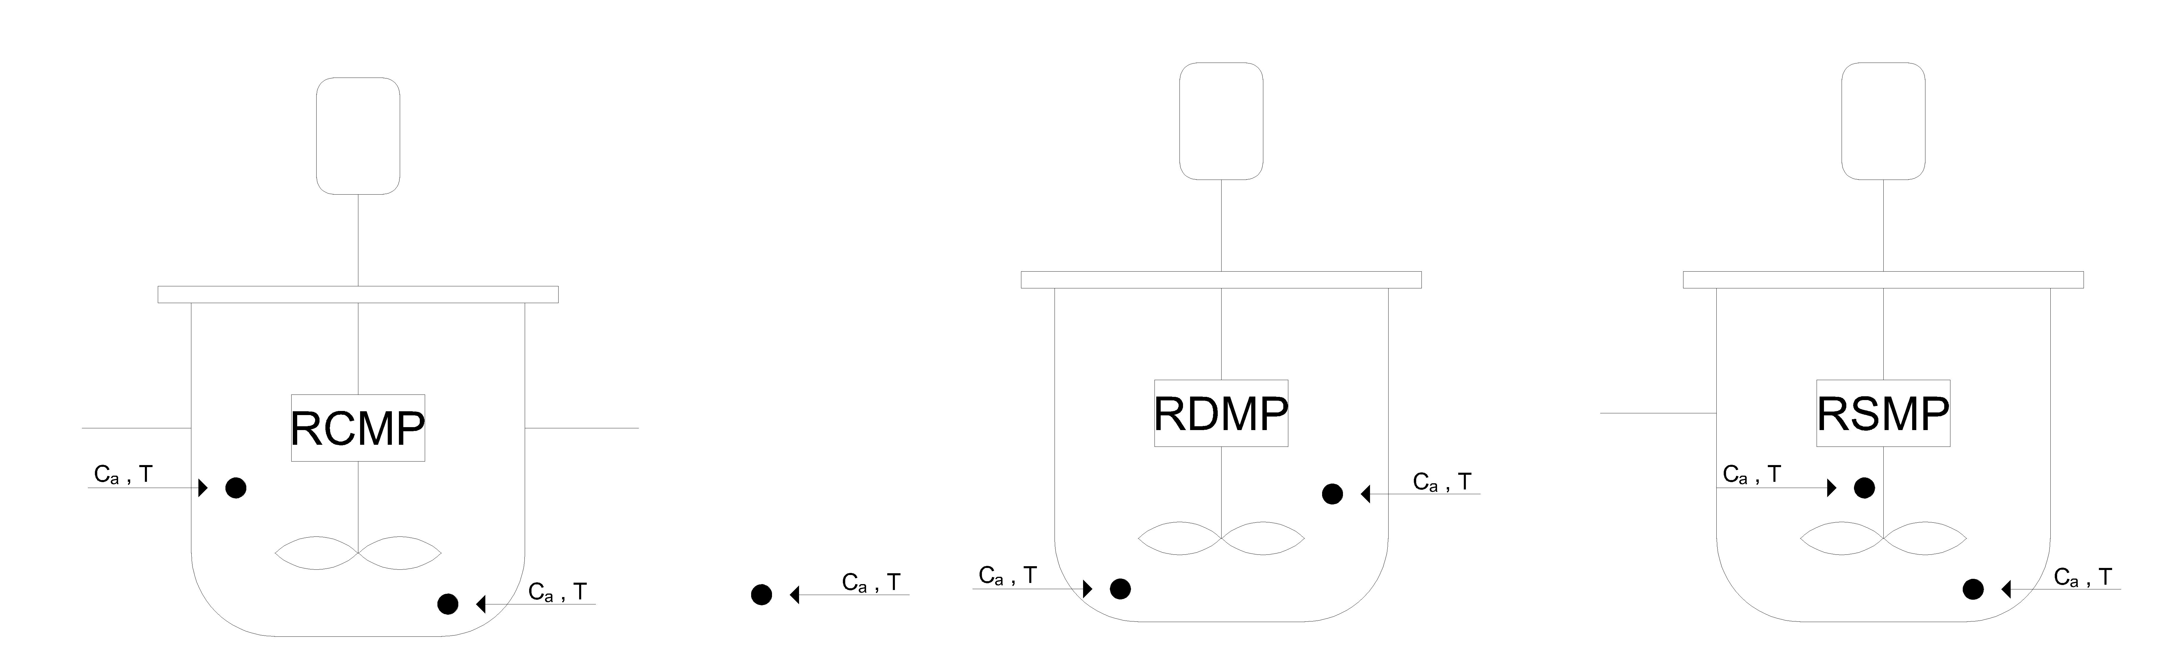
\includegraphics[width=1\textwidth]{RMP.PNG}

\subsection{Reactor de flujo piston}
\begin{raggedright}
En el reactor flujo de piston no hay mezcla a nivel axial, por tanto vamos a tener perfiles de temperatura y concentracion en funcion de la posicion en el reactor(Z).
por ello es necesario trabajar en estado estacionario, con dv al contrario de mezcla perfecta que siempre trabajamos con V, ademas obviamente solo se puede trabajar en continuo.
\end{raggedright}
\begin{center}
	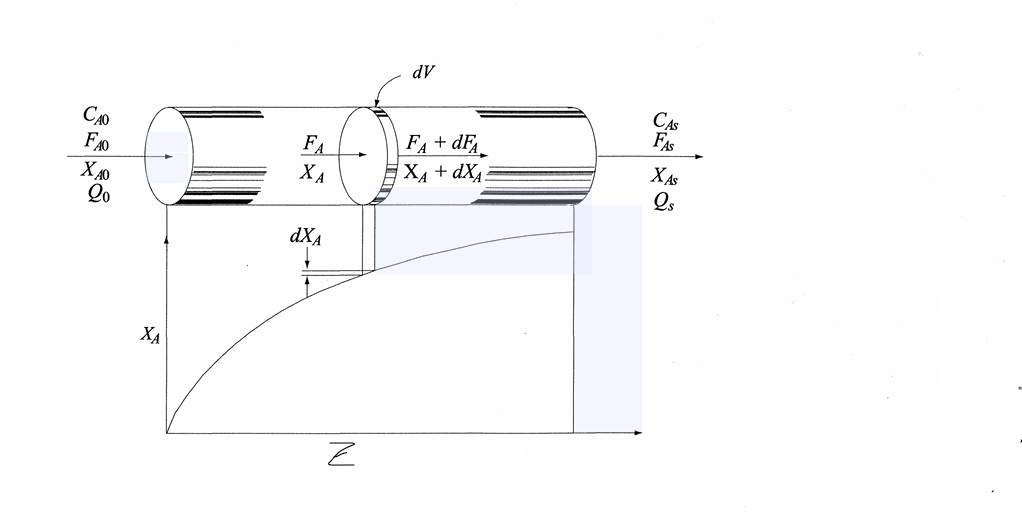
\includegraphics[width=0.8\textwidth]{RFP.png}
\end{center}

\section{Modelizacion de reactores}
\subsection{Modelo de mezcla perfecta}
\begin{raggedright}
	\vspace{1\baselineskip}
	\noindent \textbf{Balance global en continuo:}
	\begin{equation}
		\frac{dM}{dt}=m_o-m_s
	\end{equation}
	si la masa la establecemos en funcion del volumen se puede establecer con el caudal volumetrico y densidad:
	\begin{equation}
		\frac{d(V\rho)}{dt}=F_o\rho_o-F_s\rho_s
	\end{equation}
	en el caso de trabajar en condiciones isomtermas $\rho$ es constante, y en caso de que trabajemos en un rango pequeño de temperatura podemos considerar un valor medio tal que:
	\begin{equation}
		\frac{dV}{dt}=F_o-F_s \xleftrightarrow{\text{V=cte}} \sum F_o=\sum F_s
	\end{equation}
	De forma que el caudal volumetrico de entrada coincide con el caudal volumetrico de salida.
\end{raggedright}
\nt{Esto solo se cumple cuando trabajamos en un reactor ideal ya que se supone mezcla perfecta,un buen sistema de agitacion que cumple las condiciones de homogeniedad y que mantenga un volumen constante.
 en caso contrario  regulando por control de nivel se varia el acceso de corriente de entrada o de salida se mantenga en volumen constante}
 
\vspace{1\baselineskip}
\noindent \textbf{Balance a componentes:}
 \begin{equation}
	 \frac{dN_i}{dt}=ni_o-ni_s +ri \cdot V
 \end{equation}
\begin{flushleft}
\noindent es decir la variacion del numero de moles del componente i respecto al tiempo es igual a la diferencia de moles de entrada y salida mas la velocidad de reacción del componente i por el volumen del reactor (Termino de generacion).\\

 a su vez aunque debemos trabajar en moles puesto que estamos en una reacción quimica, nos interesa mas trabajar en concentraciones ya que nos da mucha mas informacion, y como
 $V\cdot C_i =N_i$ podemos reescribir la ecuacion anterior de la siguiente forma:

\end{flushleft}
 \begin{equation}
	 \frac{d(C_i\cdot V)}{dt}=C_{io}\cdot F_o-C_{is}\cdot F_s +r_i \cdot V
 \end{equation}
\begin{flushleft}

\noindent de donde como se ha mencionado anteriormente, V al ser constante puede salir de la derivada, el caudal volumetrico de entrada es igual al de salida (1.3), ademas como estamos en una mezcla perfecta.\\ 
La concentracion en la entrada y salida del reactor deben de ser identicas ya que para ser una mezcla perfecta en cualquier punto del reactor debe tener las mismas propiedades $\rightarrow C_i=C_{is}$, por tanto se simplifica a la siguiente ecuacion:

\end{flushleft}
 \begin{equation}
	V\frac{dC_i}{dt}=F\cdot (C_{io}-C_{is}) +V \cdot r_i \hspace{0.2cm}\xleftrightarrow{\;\qquad} \hspace{0.2cm}\frac{dC_i}{dt}=\frac{F}{V}\cdot (C_{io}-C_{is}) +r_i
 \end{equation}
 \noindent F/V tambien se define como el tiempo de residencia $\tau$ del reactor, es decir el tiempo que una particula pasa en el reactor.
\newpage
\vspace{1\baselineskip}
\noindent \textbf{Balance de energía:}
\begin{flushleft}
	\noindent el balance, se trata fundamentalmente de un balance entalpico, es decir si estamos en un proceso endotermico dara una disminucion de la temperatura y si es exotermico un aumento de la temperatura.\\
\end{flushleft}
\clm{}{}{	\begin{equation}
	\sum_{i=A}^{P} (M_i \cdot C_{pi}) \cdot \frac{dT}{dt} = \sum_{i=A}^{P} (F_o \cdot C_{io} \cdot H_{io}) - F_s \cdot C_{is} \cdot H_{is} + V \cdot \sum_{k=1}^{n} \Delta H_k \cdot r_k + Q(T)
\end{equation}}

\begin{flushleft}
	\noindent donde la variacion de energia, se puede calcular como la sumatoria para cada componente de su masa por su capacidad calorifica por la variacion de temperatura respecto del tiempo, es decir es el termino de acumulacion.

\vspace{1\baselineskip}
el termino de entalpia de entrada - el de salida de los componentes se trata de $ \sum_{i=A}^{P} (F_o \cdot C_{io} \cdot H_{io}) - F_s \cdot C_{is} \cdot H_{is}$\\
\vspace{1\baselineskip}
mientras que el termino de generación a diferencia del anterior depende de las reacciones quimica, de ahi que sea el indice k frente al i que era de los componentes.
\begin{equation*}
	V \cdot \sum_{k=1}^{n} \Delta H_k \cdot r_k
\end{equation*}
cada reacción tendra su propia entalpia,la entalpia tiene unidad de J|Kj /mol por ello debe ir multiplicada a la velocidad de reacción referida al mismo componente, de forma que queda unidad de energia/(tiempo*V) por ello es necesario multiplicar el volumen \\
\vspace{1\baselineskip}
por ultimo el termino Q(T) es el termino de intercambio de calor, que salvo que trabajemos en condiciones adiabaticas (para el diseño principalmente) siempre ha de estar.

teniendo en cuenta la expresion general, para poder trabajar con ello hay que tener en cuenta que al estar en ideal,mezcla perfecta se tienen las siguientes consideraciones:
\end{flushleft}
\begin{enumerate}[label=\bfseries\tiny\protect\circled{\small\arabic*}]
\item \label{n:1} T = $T_s$
\item \label{n:2} $\rho$ $\approx$ cte ,\hspace{0.1cm} $\rho$ = $\sum_{i=A}^{P} c_i$
\item \label{n:3} $cp_i$ $\approx$ valores medios, cp
\item \label{n:4} V$\cdot$ $\rho$ = M
\item \label{n:5} en sistemas a presion constante, $\Delta H$ = Cp*T y como en la ecuacion es entrada-salida, $\Delta H$ = Cp*(T$_o$-T$_s$)
\end{enumerate}
es decir nos quedaria la siguiente expresion:
\begin{equation}
	V \cdot \rho \cdot cp \cdot \frac{dT}{dt} = F \cdot  \rho \cdot cp \cdot (T_o - T_s) + V \cdot \sum_{k=1}^{n} \Delta H_k \cdot r_k + Q(T)
\end{equation}
simplificando:
\begin{equation}
	\frac{dT}{dt} = \frac{F}{V} \cdot (T_o - T_s) +  \sum_{k=1}^{n} \frac{\Delta H_k \cdot r_k}{\rho \cdot cp} + \frac{Q(T)}{V \cdot \rho \cdot cp}
\end{equation}
\newpage

\subsection{velocidades de reacción}
\vspace{1\baselineskip}
\qs{Calculo de velocidades de reacción}{ 
\schemestart
A + B \arrow{->[1]} C + D \arrow{<->[3]} F
\arrow(@c2--){->[\rotatebox{90}{2}]}[-90] 2E  % Flecha hacia abajo desde C + D
\schemestop}
\sol $r_k$ velocidades de reacción:
\begin{itemize}
	\item $r_1 = k_1 \cdot C_A \cdot C_B$
	\item $r_2 = k_2 \cdot C_C$
	\item $r_3 = k_3 \cdot C_D - k_{-3} \cdot C_F$
\end{itemize}
\sol $r_i$, velocidades de compontentes:
\begin{multicols}{2} % Dividir en 2 columnas
	\begin{itemize}
		\item $r_A = -r_1$
		\item $r_B = -r_1$
		\item $r_C = r_1 - \frac{r_2}{2}$
		\item $r_D = r_1 - r_3$
		\item $r_F = r_3$
		\item $r_E = r_2$
	\end{itemize}
	\end{multicols}

\nt{Las velocidades de reacción, va dirigada a uno de los componentes, normalmente en funcion del producto o del reactivo limitante, Vienen expresadas en terminos de moles/(tiempo*V)}
\subsubsection{Fase Líquida}
la velocidad de reaccion esta en funcion de la constante cinetica (que sera en funcion de la temperatura y de las concentracionees) por tando:
\begin{equation}
	r = f(k,c_i) \rightarrow r=f(T,X_A)
\end{equation}
a su vez, la constante cinetica se obtiene mediante Arrhenius:
\begin{equation}
	k = k_0 \cdot \exp\left(\frac{-E_A}{RT}\right)
\end{equation}
y recordando expresando en funcion de la conversion se puede operar de la siguiente forma:
\begin{equation}
	X_A = \frac{N_{AR}-N_A}{N_{AR}} \rightarrow N_A = N_{AR} \cdot (1-X_A)
\end{equation}
\begin{equation*}
	N_A = f(X_A) \approx C_A = f(X_A)
\end{equation*}
por tanto la concentracion inicial es:
\begin{equation}
	C_{i} = C_{io} - \frac{\alpha_i}{\alpha_A} \cdot (X_A-X_{Ao})
\end{equation}
Siendo $\alpha_i$ el coeficiente estequiometrico del componente i, y $\alpha_A$ el coeficiente estequiometrico del componente que se tomara como reactivo  ademas considerando, en el instante inicial que la conversion es 0:
\begin{equation}
	C_{i} = C_{io} - \frac{\alpha_i}{\alpha_A} \cdot C_{A0} \cdot X_A
\end{equation}
\newpage
\subsubsection{Fase Gaseosa}
En fase gaseosa tenemos 2 posibilidades de trabajo, bien en función de la constante cinetica y concentracion, como en la fase liquida, o bien en funcion de la constante cinetica y Presiones parciales de los componentes.
\begin{equation*}
	r = f(k,P_i) \rightarrow r=f(T,X_A)
\end{equation*}
\begin{equation*}
	n_i = n_{ie} - \frac{\alpha_i}{\alpha_A} \cdot n_{AR} \cdot (X_A-X_{Ae})
\end{equation*}
Recordando que al ser un gas ocupa todo el volumen y segun la ley de los gases ideales:
\begin{equation}
	F = \frac{R \cdot T \cdot n_t}{P}
\end{equation}
donde el numero de moles se relaciona con las presiones de la siguiente forma:
\begin{equation}
	n_t = \sum n_i \rightarrow c_i = \frac{n_i}{F} = \frac{n_i}{n_t}-\frac{P}{R \cdot T} = y_i \cdot \frac{P}{R \cdot T}
\end{equation}
A su vez aplicando la ley de Dalton para las presiones parciales:
\begin{equation}
	P_i = y_i \cdot P = \frac{n_i}{n_t} \cdot P
\end{equation}
es decir sera su fracción molar por la presion total del reactor.
\subsubsection{Calor intercambiado con el exterior}
en un intercambiador de calor, podriamos encontrarno varios casos, bien que solo se intercambie el calor lantente es decir, que no haya variacion de temperatura ya que es solo el cambio de estado, o bien que se intercambie calor sensible, es decir que haya variacion de temperatura.
tambien podria ser una combinacion de ambas.
\begin{itemize}
	\item Intercambio de calor lantente: $T_j \approx cte$ $T_j$ se trata del calor de camisa, de forma que se puede cuantificar como $Q = U\cdot S \cdot (T-T_j)$ es decir se trata del coeficiente global de transferencia de calor por la superficie de intercambio por la diferencia de temperaturas entre el reactor y su camisa.
	\item []el coeficiente de intercambio de calor U, es función de los coeficientes individuales de la transferencia de calor y conductividad termica $U = f(h_i,h_e,k)$
	\item Intercambio de calor sensible: $T_j \neq cte$ en este caso el intercambio de calor se cuantifica como la masa del fluido refrigerante por el calor especifico del mismo por la variacion de temperatura. $Q = m_j \cdot c_{pj} \cdot (T_{js}-T_{je})$
	\item []tambien se podria expresar de forma analoga al intercambio de calor latente pero con la media logaritmica, es decir $Q = U\cdot S \cdot \Delta T_{mlg}$
\end{itemize}
como lo normal es conocer la masa del fluido refrigerante y la temperatura de entrada pero no la de salida se deben correlacionar las ecuaciones anteriores.
\begin{note}
	recordando que la media logaritmica es (la mayor diferencia - la menor diferencia)/ln(mayor/menor) y por logica debe ser menor en la salida que en la entrada.
	\begin{equation*}
		Q = U \cdot S \cdot \frac{(T-T_{je})-(T-T_{js})}{\ln\left(\frac{T-T_{je}}{T-T_{js}}\right)}
	\end{equation*}
\end{note}
\noindent ahora como nos faltaria algun dato para operar con las ecuaciones previas, la forma de correlacionar ambas es la siguiente:
\newpage
\begin{proof}
	\begin{equation*}
		 Q = U\cdot S \cdot (T_{js}-T_{je})
	\end{equation*}\\
	\begin{equation*}
		U \cdot S \cdot \frac{(T{js}-T_{je})}{\ln\left(\frac{T-T_{je}}{T-T_{js}}\right)}
   \end{equation*}
\vspace{0.1cm}
	\begin{equation*}
		m_j \cdot c_{pj} \cdot (T_{js}-T_{je}) = U \cdot S \cdot \frac{(T-T_{je})-(T-T_{js})}{\ln\left(\frac{T-T_{je}}{T-T_{js}}\right)}
	\end{equation*}
	\begin{equation*}
		\ln \left(\frac{T-T_{je}}{T-T_{js}}\right) = \frac{U \cdot S }{m_j \cdot c_{pj}} 
	\end{equation*}\\

	\noindent donde simplemente despejando  de esta ultima ecuación:
	\begin{equation*}
		\frac{T-T_{je}}{T-T_{js}} = \exp\left(\frac{U \cdot S }{m_j \cdot c_{pj}}\right)
	\end{equation*}
	\begin{equation*}
		T - T_{je} = (T-T_{js}) \cdot \exp\left(\frac{U \cdot S }{m_j \cdot c_{pj}}\right) 
	\end{equation*}\\
	al pasar el exponente al otro lado de la ecuacion:\\
	\begin{equation*}
		T-T_{js} = (T - T_{je}) \cdot \exp\left(- \hspace{0.5em}\frac{U \cdot S }{m_j \cdot c_{pj}}\right) 
	\end{equation*}
	\begin{equation*}
		T_{js} = T- (T - T_{je}) \cdot \exp\left(- \hspace{0.5em}\frac{U \cdot S }{m_j \cdot c_{pj}}\right) 
	\end{equation*}
	\noindent y reintroduciendo en la primera expresion queda tal que:
	\begin{equation*}
		Q = m_j \cdot c_{pj} \cdot \left(T_{js} - \left[ T - (T - T_{je}) \cdot \exp\left(- \hspace{0.5em}\frac{U \cdot S }{m_j \cdot c_{pj}}\right) \right] \right)
	\end{equation*}
	\begin{equation*}
		Q = m_j \cdot c_{pj} \cdot (T - T_{je}) \cdot \left[1 - \exp\left(-\hspace{0.5em} \frac{U \cdot S}{m_j \cdot c_{pj}}\right)\right]
	\end{equation*}
\end{proof}
\newpage
\chapter{Reactor Discontinuo Mezcla perfecta}
\nt{\begin{raggedright}
	en un reactor biologico tenemos que f/v velocidad de dilucion (D)mientras que en otros es v/f , en el primer caso es por que se tiene
	en cuenta los caudales de salida frente los otros son de entrada, tiempos de residencia corto, en el segundo caso es tiempo espacia,
	teniendo en cuenta los caudales de entrada
\end{raggedright}}
\subsection{Isotermo}
\begin{raggedright}
	\textbf{Balance de materia:}
	\begin{equation}
		\frac{dN_i}{dt} = r_i \cdot V
	\end{equation}
	\textbf{Balance de energía:}
	\begin{equation}
		\frac{dT}{dt} = \frac{\sum_{k=1}^{n} \Delta H_k \cdot r_k}{\rho \cdot cp} + \frac{Q(T)}{V \cdot \rho \cdot cp}
	\end{equation}
\textbf{2 posibles cuestiones}
\begin{itemize}
	\item \textbf{Calculo de Volumen:} V
	\item \textbf{Calculo de Tiempo de residencia:} $\tau = \frac{V}{F}$
\end{itemize}
Dentro de los reactivos uno sera el limitante, en la etapa de diseño va referida al reactivo limitante (A)
\textbf{Refiriendonos a la conversion puesto que es el parametro que mas informacion nos da:}
ya que queremos un $\%$ minimo de conversion, se puede calcular como:
\begin{equation}
	X_A = \frac{N_{AR}-N_A}{N_{AR}} \rightarrow N_A = N_{AR} \cdot (1-X_A)
\end{equation}
en la etapa de diseño la masa dara el volumen y el balance entalpico como la temperatura es constante dara el diseño del intercambiador de calor.
por tanto el objetivo a calcular es el tiempo de residencia.
\begin{equation}
	\frac{dN_A}{dt} = -r_A \cdot V
\end{equation}
pars transformar en conversion:
\begin{equation}
	X_A = \frac{N_{AR}-N_A}{N_{AR}} \rightarrow N_A = N_{AR} \cdot (1-X_A)
\end{equation}
\begin{equation}
	\frac{dN_{AR}dX_A}{dt} = r_A \cdot V
\end{equation}
\begin{equation}
	\frac{dX_A}{dt} = \frac{r_A \cdot V}{N_{AR}}
\end{equation}
\begin{equation}
	NAR \int_{XA0}^{XA} \frac{dX_A}{r_A \cdot V} = t_R = NAR \int_{XA0}^{XA} \frac{dXA}{ra V}
\end{equation}
2 casos 
\begin{itemize}
	\item Fase liquida v =cte 
	\begin{equation}
		Tr = CAR \int_{XA0}^{XA} \frac{dxa}{ra}
	\end{equation}
	\item para fase gaseosa 
	\begin{equation}
		Tr = CAR \int_{XA0}^{XA} \frac{dxa}{ra \cdot (1 + eA + ra)}
	\end{equation}
	\end{itemize}
\end{raggedright}
\nt{V  = VR (1 + CA + XA)}
\mlenma{Para componentes que no sean referencia}{CB = CB0 -CA0 * XA \\
en el TR el divisior ra seria k1 * CA que era CA0(1-xA)* lo definido arriba}
\begin{raggedright}
	\textbf{Funcionamiento:}
\nt{Productividad = moles producto deseado /m3/s el tiempo de productividad depende del ciclo no es el de operacion del reactor sino que
incluye el de limpieza acondicionado llenado..}
Si ya esta diseñado y quiero que responda al funcionamiento y no al disño del reactor ci = f(t)
\begin{equation}
	\frac{dCA}{dt} = ra
\end{equation}

\begin{equation}
	\frac{dCB}{dt} = rb
\end{equation}

\begin{equation}
	\frac{dCC}{dt} = rc
\end{equation}
%! Eso para todos los balances ponerlo mas tarde en un multicol...
teniendo V conocido que viene de la etapa de diseño y esta construido el intercambiador de calor y conociendo los parametros Tj T..
La T define las constantes del proceso es decir las K que tambien seran conocidas.
es decir el modelo se completa conociendo r1,r2,r3,ra,rb,rc....rf tambien se puede deducir de forma implicita que simplemente con
los balances a f metiendo las cineticas de r1...r3 aunque recomienda ser explicito para luego poder variar el estudio del sistema.
\subsubsection{Analisis de varibles}
serian 15 ecuaciones las 6 de los componentes las 3 de reacciones y las 6 de los balances, el numero de variables. todas las concentraciones
todas las r y las constantes es decir k1 k2 k3 y k-3 
numero de grados de libertad 4 es decir debe conocerse las 4 constantes cineticas a esa temperatura

\end{raggedright}
% \ex{Open Set and Close Set}{}
% \thm{}{If $x\in$ open set $V$ then $\exists$ $\delta>0$ such that $B_{\delta}(x)\subset V$}
% \begin{myproof}
% \end{myproof}

% \cor{}{By the result of the proof, we can then show...}
% \mlenma{}{Suppose $\vec{v_1}, \dots, \vec{v_n} \in \RR[n]$ is subspace of $\RR^n$.}
% \mprop{}{$1 + 1 = 2$.}

% \section{Random}
% \dfn{Normed Linear Space and Norm $\boldsymbol{\|\cdot\|}$}{Let $V$ be a vector space over $\bbR$ (or $\bbC$). A norm on $V$ is function $\|\cdot\|\ V\to \bbR_{\geq 0}$ satisfying \begin{enumerate}[label=\bfseries\tiny\protect\circled{\small\arabic*}]
% 		\item \label{n:1}$\|x\|=0 \iff x=0$ $\forall$ $x\in V$
% 		\item \label{n:2}	$\|\lambda x\|=|\lambda|\|x\|$ $\forall$ $\lambda\in\bbR$(or $\bbC$), $x\in V$
% 		\item \label{n:3} $\|x+y\| \leq \|x\|+\|y\|$ $\forall$ $x,y\in V$ (Triangle Inequality/Subadditivity)
% 	\end{enumerate}And $V$ is called a normed linear space.

% 	$\bullet $ Same definition works with $V$ a vector space over $\bbC$ (again $\|\cdot\|\to\bbR_{\geq 0}$) where \ref{n:2} becomes $\|\lambda x\|=|\lambda|\|x\|$ $\forall$ $\lambda\in\bbC$, $x\in V$, where for $\lambda=a+ib$, $|\lambda|=\sqrt{a^2+b^2}$ }


% \ex{$\bs{p-}$Norm}{\label{pnorm}$V={\bbR}^m$, $p\in\bbR_{\geq 0}$. Define for $x=(x_1,x_2,\cdots,x_m)\in\bbR^m$ $$\|x\|_p=\Big(|x_1|^p+|x_2|^p+\cdots+|x_m|^p\Big)^{\frac1p}$$(In school $p=2$)}
% \textbf{Special Case $\bs{p=1}$}: $\|x\|_1=|x_1|+|x_2|+\cdots+|x_m|$ is clearly a norm by usual triangle inequality. \par
% \textbf{Special Case $\bs{p\to\infty\ (\bbR^m$ with $\|\cdot\|_{\infty})}$}: $\|x\|_{\infty}=\max\{|x_1|,|x_2|,\cdots,|x_m|\}$\\
% For $m=1$ these $p-$norms are nothing but $|x|$.
% Now exercise
% \qs{}{\label{exs1}Prove that triangle inequality is true if $p\geq 1$ for $p-$norms. (What goes wrong for $p<1$ ?)}
% \sol{\textbf{For Property \ref{n:3} for norm-2}	\subsubsection*{\textbf{When field is $\bbR:$}} We have to show\begin{align*}
% 		         & \sum_i(x_i+y_i)^2\leq \left(\sqrt{\sum_ix_i^2} +\sqrt{\sum_iy_i^2}\right)^2                                       \\
% 		\implies & \sum_i (x_i^2+2x_iy_i+y_i^2)\leq \sum_ix_i^2+2\sqrt{\left[\sum_ix_i^2\right]\left[\sum_iy_i^2\right]}+\sum_iy_i^2 \\
% 		\implies & \left[\sum_ix_iy_i\right]^2\leq \left[\sum_ix_i^2\right]\left[\sum_iy_i^2\right]
% 	\end{align*}So in other words prove $\langle x,y\rangle^2 \leq \langle x,x\rangle\langle y,y\rangle$ where
% 	$$\langle x,y\rangle =\sum\limits_i x_iy_i$$

% 	\begin{note}
% 		\begin{itemize}
% 			\item $\|x\|^2=\langle x,x\rangle$
% 			\item $\langle x,y\rangle=\langle y,x\rangle$
% 			\item $\langle \cdot,\cdot\rangle$ is $\bbR-$linear in each slot i.e. \begin{align*}
% 				      \langle rx+x',y\rangle=r\langle x,y\rangle+\langle x',y\rangle	\text{ and similarly for second slot}
% 			      \end{align*}Here in $\langle x,y\rangle$ $x$ is in first slot and $y$ is in second slot.
% 		\end{itemize}
% 	\end{note}Now the statement is just the Cauchy-Schwartz Inequality. For proof $$\langle x,y\rangle^2\leq \langle x,x\rangle\langle y,y\rangle $$ expand everything of $\langle x-\lambda y,x-\lambda y\rangle$ which is going to give a quadratic equation in variable $\lambda $ \begin{align*}
% 		\langle x-\lambda y,x-\lambda y\rangle & =\langle x,x-\lambda y\rangle-\lambda\langle y,x-\lambda y\rangle                                       \\
% 		                                       & =\langle x ,x\rangle -\lambda\langle x,y\rangle -\lambda\langle y,x\rangle +\lambda^2\langle y,y\rangle \\
% 		                                       & =\langle x,x\rangle -2\lambda\langle x,y\rangle+\lambda^2\langle y,y\rangle
% 	\end{align*}Now unless $x=\lambda y$ we have $\langle x-\lambda y,x-\lambda y\rangle>0$ Hence the quadratic equation has no root therefore the discriminant is greater than zero.

% 	\subsubsection*{\textbf{When field is $\bbC:$}}Modify the definition by $$\langle x,y\rangle=\sum_i\overline{x_i}y_i$$Then we still have $\langle x,x\rangle\geq 0$}

% \section{Algorithms}
% \begin{algorithm}[H]
% \KwIn{This is some input}
% \KwOut{This is some output}
% \SetAlgoLined
% \SetNoFillComment
% \tcc{This is a comment}
% \vspace{3mm}
% some code here\;
% $x \leftarrow 0$\;
% $y \leftarrow 0$\;
% \uIf{$ x > 5$} {
%     x is greater than 5 \tcp*{This is also a comment}
% }
% \Else {
%     x is less than or equal to 5\;
% }
% \ForEach{y in 0..5} {
%     $y \leftarrow y + 1$\;
% }
% \For{$y$ in $0..5$} {
%     $y \leftarrow y - 1$\;
% }
% \While{$x > 5$} {
%     $x \leftarrow x - 1$\;
% }
% \Return Return something here\;
% \caption{what}
% \end{algorithm}
% \chapter{2}
\end{document}
